%%%%%%%%%%%%%%%%%%%%%%%%%%%%%%%%%%%%%%%%%
% Beamer Presentation
% LaTeX Template
% Version 1.0 (10/11/12)
%
% This template has been downloaded from:
% http://www.LaTeXTemplates.com
%
% License:
% CC BY-NC-SA 3.0 (http://creativecommons.org/licenses/by-nc-sa/3.0/)
%
%%%%%%%%%%%%%%%%%%%%%%%%%%%%%%%%%%%%%%%%%

%----------------------------------------------------------------------------------------
%	PACKAGES AND THEMES
%----------------------------------------------------------------------------------------

\documentclass[14pt]{beamer}

\mode<presentation> {

% The Beamer class slide themes
\usetheme{Madrid} %i was using this one

% Beamer class color themes

%\usecolortheme{albatross}

%\setbeamertemplate{footline} % To remove the footer line in all slides uncomment this line
%\setbeamertemplate{footline}[page number] % To replace the footer line in all slides with a simple slide count uncomment this line

%\setbeamertemplate{navigation symbols}{} % To remove the navigation symbols from the bottom of all slides uncomment this line
}

\usepackage{graphicx} % Allows including images
\usepackage{booktabs} % Allows the use of \toprule, \midrule and \bottomrule in tables
\usepackage{hyperref}
\usepackage{helvet}

%----------------------------------------------------------------------------------------
%	TITLE PAGE
%----------------------------------------------------------------------------------------

\title[RNAseq]{RNA Sequencing Examples} % The short title appears at the bottom of every slide, the full title is only on the title page

\author{C. Ryan Campbell} % Your name
\institute[Duke] % Your institution as it will appear on the bottom of every slide, may be shorthand to save space
{
Duke University \\ % Your institution for the title page
\medskip
\textit{c.ryan.campbell@duke.edu} % Your email address
}
\date{3 Oct 2017} % Date, can be changed to a custom date

\begin{document}

\begin{frame}
\titlepage % Print the title page as the first slide
\end{frame}

\begin{frame}
\frametitle{Overview} % Table of contents slide, comment this block out to remove it
\tableofcontents % Throughout your presentation, if you choose to use \section{} and \subsection{} commands, these will automatically be printed on this slide as an overview of your presentation
\end{frame}

%----------------------------------------------------------------------------------------
%	PRESENTATION SLIDES
%----------------------------------------------------------------------------------------

%------------------------------------------------
\section{Goals} 
%------------------------------------------------

%------------------------------------------------
\begin{frame}
\frametitle{Today's Goals}
%what students should know/learn today
\begin{itemize}
	\item<+-> What are RNAseq best practices?
	\item<+-> How did the assigned papers address these recommendations?
	\item[]
	\item<+-> Jigsaw Activity
\end{itemize}
\end{frame}

%------------------------------------------------
\begin{frame}
\frametitle{Review to Read}
\begin{itemize}
	\item<+-> This is a summary from:
	\item<+-> Conesa et al. 2016. A survey of best practices for RNA-seq data analysis.
	\item<+-> Good overview of current ``best practices''
\end{itemize}
\end{frame}

%------------------------------------------------
\begin{frame}
\frametitle{Jigsaw Activity}
\begin{itemize}
	\item<+-> Each of your papers took a different approach to this problem
	\item<+-> As I'm covering these practices make a note of what your paper did
	\item<+-> Compare and contrast during the activity
\end{itemize}
\end{frame}

%------------------------------------------------
\section{Experimental Design}
%------------------------------------------------
%going beyond just "experiment" and "control"
%------------------------------------------------
\begin{frame}
\frametitle{Experimental Design}
\begin{itemize}
	\item<+-> Enrichment method
	\begin{itemize}
		\item<+-> Deplete rRNA 
		\item<+-> Enrich mRNA via polyA selection
	\end{itemize}
	\item<+-> Library Type (single v paired-end)
	\item<+-> Sequencing Depth
	\item<+-> Number of Replicates
\end{itemize}
\end{frame}

%------------------------------------------------
\begin{frame}
\frametitle{Enrichment}
\begin{itemize}
	\item<1-> Deplete rRNA
	\begin{itemize}
		\item<3-> Requires good quality RNA
		\item<4-> High RIN (RNA Integrity Number)
		\item<5-> Often not possible with tissue
	\end{itemize}
	\item<2-> Enrich mRNA via polyA selection
	\begin{itemize}
		\item<6-> Have to use with bacterial samples (lack polyA)
	\end{itemize}	
\end{itemize}
\end{frame}

%------------------------------------------------
\begin{frame}
\frametitle{Library Type}
\begin{itemize}
	\item<1-> Single End
	\begin{itemize}
		\item<3-> Better for well-annotated organisms
		\item<4-> Cost can go towards more reads, better coverage
	\end{itemize}
	\item<2-> Paired End
	\begin{itemize}
		\item<5-> More crucial for \textit{de novo}
		\item<6-> Improve mappability to ``dicey'' genomes
	\end{itemize}	
\end{itemize}
\end{frame}

%------------------------------------------------
\begin{frame}
\frametitle{Sequencing Depth}
\begin{itemize}
	\item<1-> Deeper is better
	\item<2-> Lower end ranges from:
	\begin{itemize}
		\item<3-> 5mil reads (for common mRNA)
		\item<4-> 100mil reads (for rare mRNA)
	\end{itemize}
	\item<5-> What else would effect necessary depth?
	%%\begin{itemize}
	%%	\item<6-> Genome complexity of the organism matter
	%%\end{itemize}
	\item<7-> Use a ``Saturation Curve'' to assess results at given depth
\end{itemize}
\end{frame}
%------------------------------------------------
\subsection{Number of Replicates}
%------------------------------------------------

%------------------------------------------------
\begin{frame}
\frametitle{Number of Replicates}
\begin{itemize}
	\item<1-> Depends on:
	\begin{enumerate}
	\item<2-> Technical Variability
	\begin{itemize}
		\item<3-> Technical replicates should result in an R-squared \texttt{>} 0.9
	\end{itemize}
	\item<4-> Biological Variability
	\item<5-> Desired Statistical Power
	\end{enumerate}
	\item<6-> Minimum of 3 replicates per group
	\item<7-> Conduct a power analysis
\end{itemize}
\end{frame}

%------------------------------------------------
\begin{frame}
\frametitle{Number of Replicates}
	\begin{center}
    	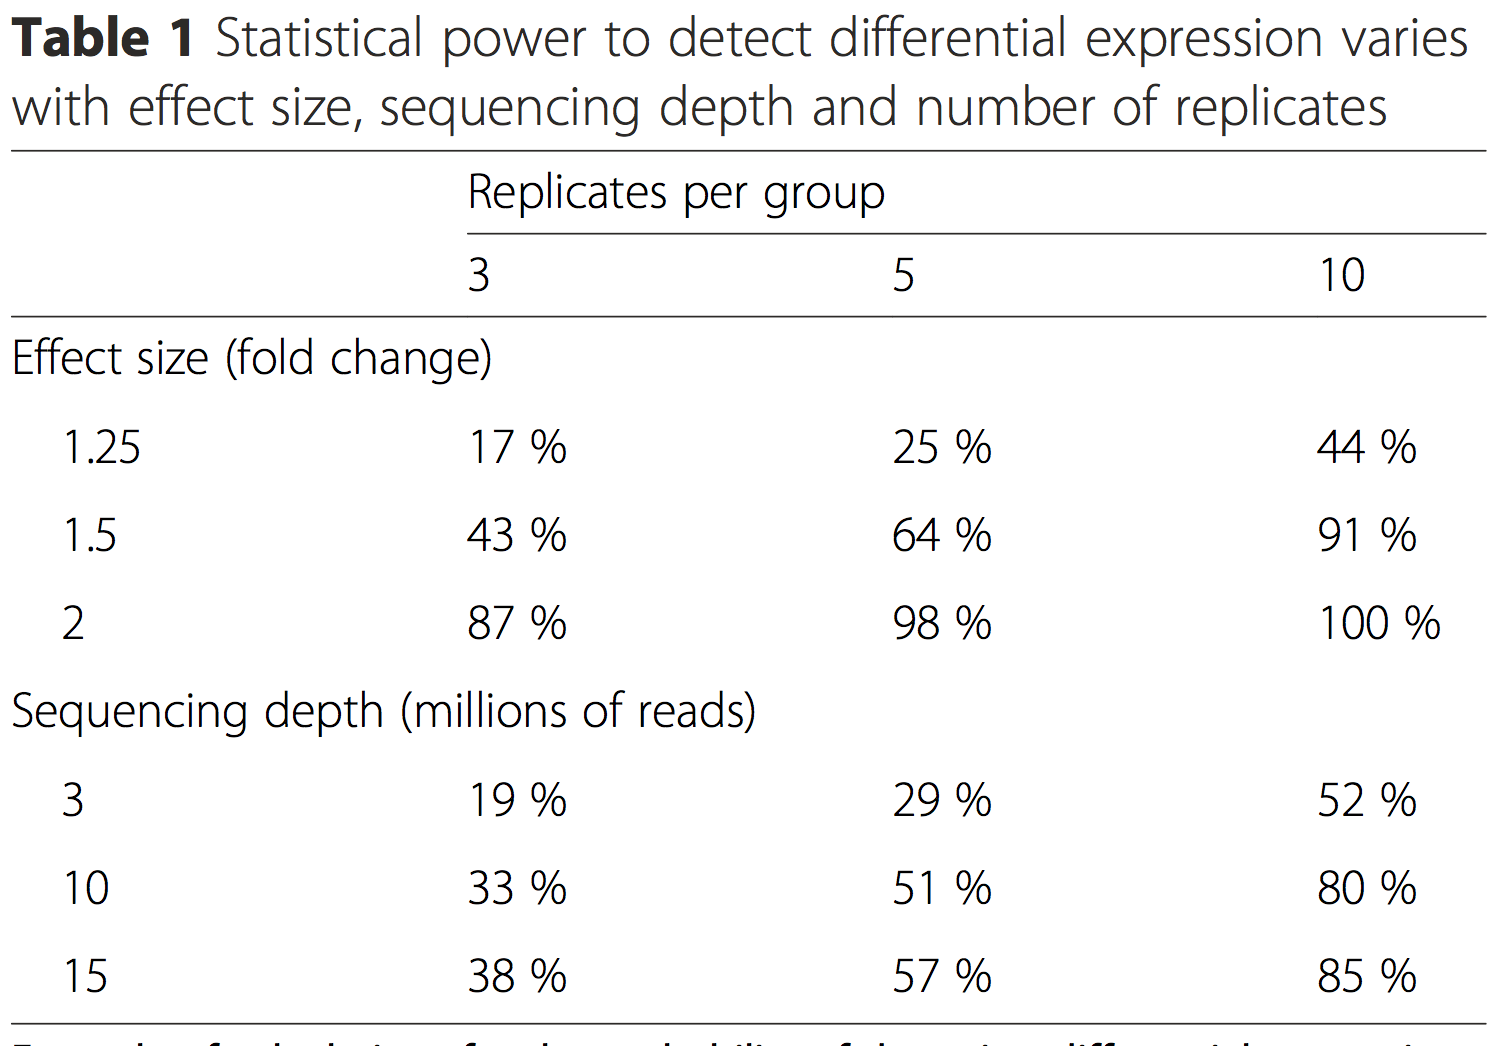
\includegraphics[width=.8\textwidth]{images_20171003_power_analysis.png}
    \end{center}
\end{frame}


%------------------------------------------------
\section{Data Analysis}
%------------------------------------------------

%------------------------------------------------
\subsection{Handling Reads}
%------------------------------------------------

%------------------------------------------------
\begin{frame}
\frametitle{Handling Reads}
\begin{itemize}
	\item<1-> Clean reads with FASTX-Toolkit or Trimmomatic
	\item<2-> Expect 70-90\% of reads aligning (model organism)
	\item<3-> Reads accumulating at the 3' end of transcripts could be a sign of poor RNA quality (polyA enrichment only)
\end{itemize}
\end{frame}

%------------------------------------------------
\subsection{Transcripts}
%------------------------------------------------
%Quantification
%------------------------------------------------
\begin{frame}
\frametitle{Transcripts}
\begin{itemize}
	\item<1-> If a genome/annotation exists you can map to it
	\item<2-> but, you can only quantify expression
	\item<3-> Discovery of new transcripts must be done separately
\end{itemize}
\end{frame}

%------------------------------------------------
\begin{frame}
\frametitle{Transcript Discovery}
\begin{itemize}
	\item<1-> Need high coverage to discvoer new transcripts
	\item<2-> Paired end data helps, hard to get complete transcript (see: IsoSeq)
	\item<3-> Several software to tackle this question:
	\item<4-> Cufflinks, iReckon, SLIDE, StringTie
	\item<5-> Montebello - quantification AND isoforms! (project idea?)
\end{itemize}
\end{frame}

%------------------------------------------------
\begin{frame}
\frametitle{Transcript Quantification}
\begin{itemize}
	\item<1-> Count transcripts to measure expression
	\item<2-> Raw counts of mapped reads are converted...
	%%\item<3-> to RPKM (reads per kilobase of exon model per million reads)
	\item<4-> Not necessary when comparing within the same gene across samples
	\item<5-> Is necessary for correctly \underline{ranking} gene expression levels
\end{itemize}
\end{frame}

%------------------------------------------------
\subsection{Differential Expression}
%------------------------------------------------

%------------------------------------------------
\begin{frame}
\frametitle{Differential Expression}
\begin{itemize}
	\item<1-> Find which genes are expressed at different levels
	\item<2-> Possible software to use:
	\item<3-> Cufflinks, TMM, DESeq, PoissonSeq, UpperQuartile
	\item<4-> COMBAT and ARSyN can be used to correct batch effects
	\item<5-> Not necessaily memory intensive software (DESeq runs in R)
\end{itemize}
\end{frame}

%------------------------------------------------
\subsection{Functional Profiling}
%------------------------------------------------

%------------------------------------------------
\begin{frame}
\frametitle{Functional Profiling}
\begin{itemize}
	\item<1-> Genes are nice, but what do they do?
	\item<2-> Characterize the function of the differentially expressed genes
	\item<3-> Also compare functional patheways for over or under-expression
	\item<4-> Tools:
	\item<5-> GOseq, Blast2GO, Gene Set Variation Analysis, SeqGSEA
\end{itemize}
\end{frame}

%------------------------------------------------
\begin{frame}
\frametitle{Jigsaw Activity}
\begin{enumerate}
	\item<+-> Form a group with everyone else who read the same paper
	\item<+-> Discuss your paper by answering the questions on the next slide -- \textbf{10-15 mins}
	\item<+-> Get together with a new group, with a single representative from each paper covered
	\item<+-> Share your results and discuss the differences -- \textbf{15-20 mins}
\end{enumerate}
\end{frame}

%------------------------------------------------
\begin{frame}
\frametitle{Jigsaw Activity}
\begin{columns}
	\begin{column}{0.4\textwidth}
		\begin{itemize}
			\item \textbf{Mouse Olf} - Sisi, Kevin, Alan
			\item \textbf{Lemurs} - Alvin, Rahul, Helena
			\item \textbf{AD} - Austin, Othmane, Jenn
			\item \textbf{Obese Chickens} - Hank, Nayib, Jake
		\end{itemize}
		\end{column}
	\begin{column}{0.6\textwidth}
		\begin{enumerate}
			\large
		\item Number (and type) of replicates
		\item Software used
		\item What functional analysis was done?
		\item What conclusions were drawn?
		\end{enumerate}
	\end{column}
\end{columns}
\end{frame}

%------------------------------------------------
\begin{frame}
\Huge{\centerline{The End}}
\end{frame}

%----------------------------------------------------------------------------------------

\end{document} 